
\pagebreak
\section{Input and Output}
Unfortunately MATLAB really falls a bit short in input and output of files.
 Their GUI file importer has improved by leaps and bounds, however.
 We'll explore a couple of different ways for file IO below.

\subsection{File Read/Write}
There is the capacity for low-level IO.
 This can be helpful when reading binar files (otherwise I would avoid it).
 TODO: Finish this section.

\begin{quote}
\verbatiminput{code/ch05_fileio.m}
\end{quote}

\pagebreak
\subsection{GUI File Read}
Matlab can automate the reading of most simple delimited text files.
 You can then copy Matlab code to automate the read later.
 This can only really be demonstrated with screnshots;

\begin{figure}[ht!]
\centering
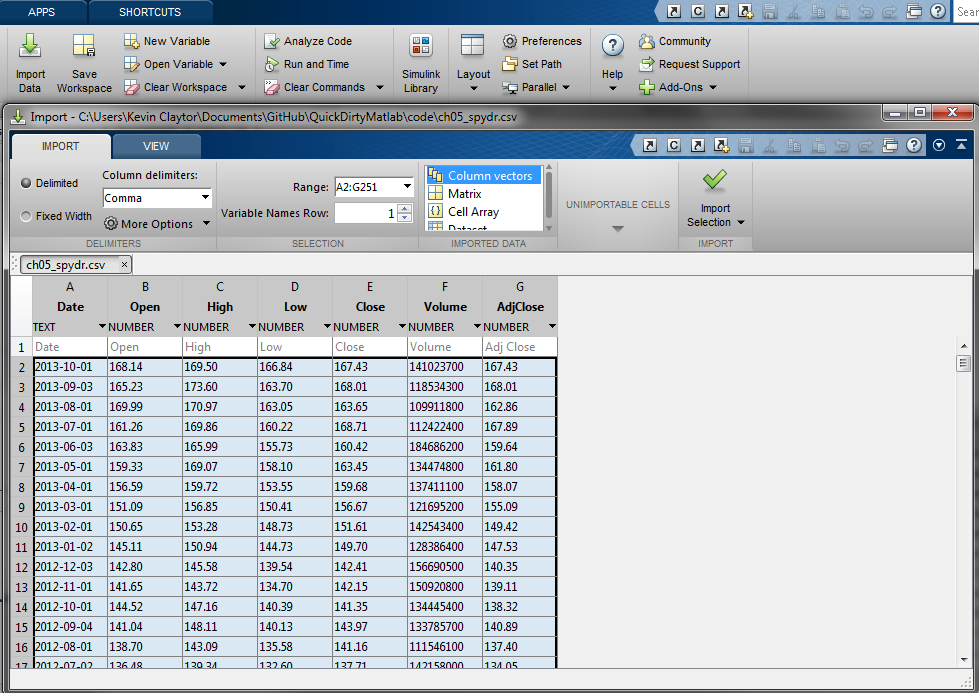
\includegraphics[width=120mm]{img/guiload.png}
\caption{The GUI file reader. From here you can select what subset of your data to import.}
\label{guiload}
\end{figure}

\pagebreak
\subsection{Save and Load}
Matlab also has \emph{save} and \emph{load} commands that allow for direct saving of multiple Matlab variables and variable types.
 This is similar to Python's pickle module.

\begin{quote}
 \verbatiminput{code/ch05_saveload.m}
\end{quote}
